\subsection{Contribución al sistema de conocimiento}
Se describen las contribuciones realizadas al sistema de conocimiento
durante los diferentes desarrollos realizados bajo el contexto del proyecto. 
Se presentan los componentes y plantillas que han sido almacenados una vez
terminado el proceso de validación y se han considerado útiles para futuros
proyectos.

\subsubsection{Plantillas}
\begin{table}[h!]
    \centering
    \begin{tabular}{| m{4cm} | m{8cm} |}
      \hline
      \textbf{Nombre de la Plantilla} & \textbf{Descripción} \\ 
      \hline
      Plantilla Básica & Configuración de infraestructura y herramientas de desarrollo.
      Crea una estructura de carpetas con varios archivos básicos. \\ 
      \hline
      XGBoost Forecasting & Adaptación de la plantilla básica a problemas de forecasting.
      Incorpora un bucle de entrenamiento que permite aplicar un modelo de forecasting sobre un dataset.\\ 
      \hline
      XGBoost Classification & Modificación de la plantilla de forecasting pero incorporando un modelo
      de clasificación.\\ 
      \hline
      Sktime Classification & Plantilla que utiliza las funcionalidades de la librería 
      Sktime para hacer una clasificación en un problema de series temporales \\ 
      \hline
      Detección de Anomalías & Plantilla base para la detección de anomalías 
      utilizando técnicas de clustering para detectar patrones anómalos.\\ 
      \hline
      AutoML Forecasting &  Plantilla que automatiza la prueba de modelos 
      de forecasting y realiza una búsqueda eficiente de hiperparámetros.\\ 
      \hline
    \end{tabular}
    \caption{Tabla de plantillas.}
    \label{table:templates}
\end{table}

\subsubsection{Componentes}
En esta subsección se presentan los componentes dibididos por categorías.
Además, se incluye una breve descripción de cada uno de ellos junto a su funcionalidad.

\paragraph{Componentes de características}
\begin{itemize}
    \item \textbf{add\_time\_features:} Añade características temporales a un conjunto de datos
    de series temporales. Se pueden añadir características como el día de la semana, el mes, el año,
    la hora, entre otros. Es necesario que el argumento de entrada sea una serie temporal con la
    columna de fecha como índice.
    \item \textbf{add\_lags:} Añade retrasos a un conjunto de datos de series temporales. Se pueden
    añadir retrasos de cualquier longitud y se puede especificar si se desea eliminar las filas con
    valores nulos. Es necesario que el argumento de entrada sea una serie temporal con la columna de
    fecha como índice.
    \item \textbf{add\_hollidays:} El componente toma como entrada un DataFrame y un objeto 
    calendario (por defecto, utiliza el calendario de los Estados Unidos) y 
    añade una columna adicional denominada \textit{holiday} que indica si la fecha es un día festivo
    o no.
\end{itemize}


\paragraph{Componentes de visualización}
\begin{itemize}
    \item \textbf{show\_time\_series\_compare:} Permite comprar el resultado de dos series temporales,
    mostrando un gráfico con ambas series. Además, se puede especificar el rango de fechas a mostrar.
    No es necesario que las series tengan la misma longitud, mientras que utilicen la columna de fecha
    como índice.
    \begin{figure}[!h]
        \centering
        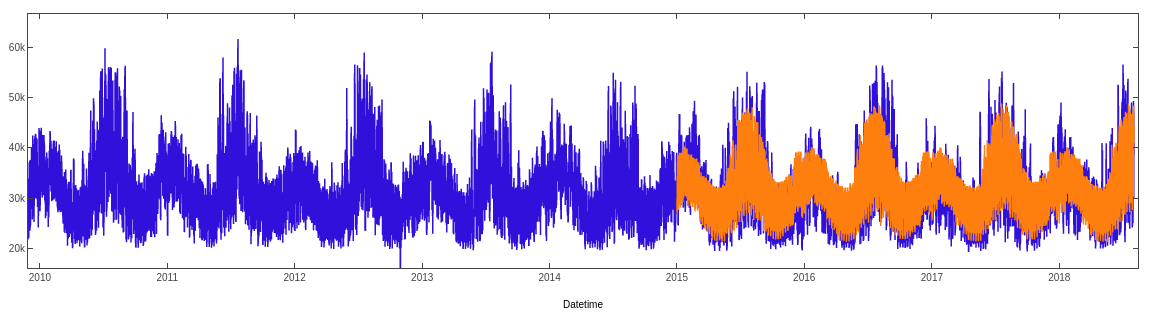
\includegraphics[width=0.8\textwidth]{compare_predictions.png}
        \caption{Previsualización del componente show\_time\_series\_compare}
        \label{fig:compare_predictions}
    \end{figure}
    \item \textbf{show\_feature\_importance:} Muestra un gráfico de barras con la importancia de las
    características de un modelo de aprendizaje automático. Se puede enviar como parámetro conjunto 
    de valores con sus respectivas etiquetas y el propio componente se encarga de realizar el gráfico
    de manera descendente en función a la relevancia de las características.
    \begin{figure}[!h]
        \centering
        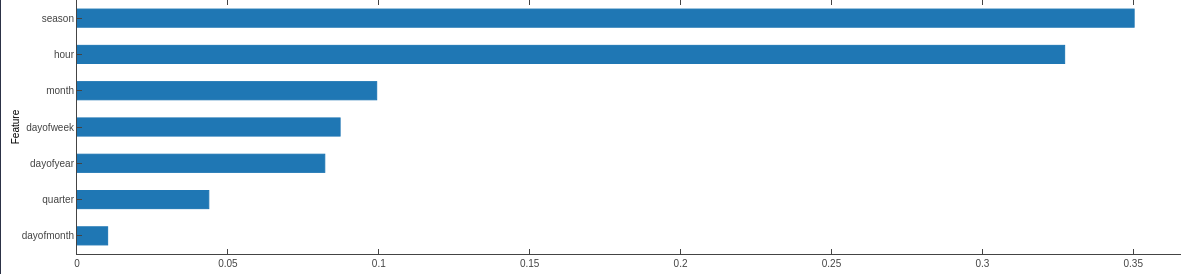
\includegraphics[width=0.6\textwidth]{feature_importance.png}
        \caption{Previsualización del componente show\_feature\_importance}
        \label{fig:feature_importance}
    \end{figure}
    \item \textbf{show\_time\_series\_outlier:} Este componente recibe como parámetros de entrada
    una serie temporal y una lista de outliers. Devuelve un gráfico de la serie temporal con los
    outliers marcados. 
    \begin{figure}[!h]
        \centering
        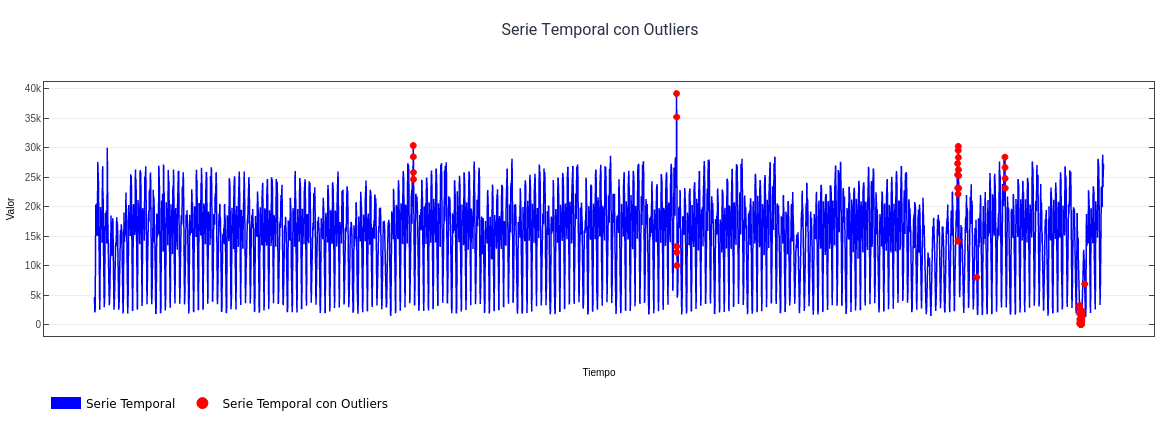
\includegraphics[width=0.8\textwidth]{outlier_component.png}
        \caption{Previsualización del componente show\_time\_series\_outlier}
        \label{fig:outlier_component}
    \end{figure}
    \item \textbf{show\_roc\_curve:} Muestra la curva ROC de un modelo de clasificación. Se puede
    enviar como parámetro el conjunto de valores reales y predichos y el componente se encarga de
    realizar el gráfico.
    \begin{figure}[!h]
        \centering
        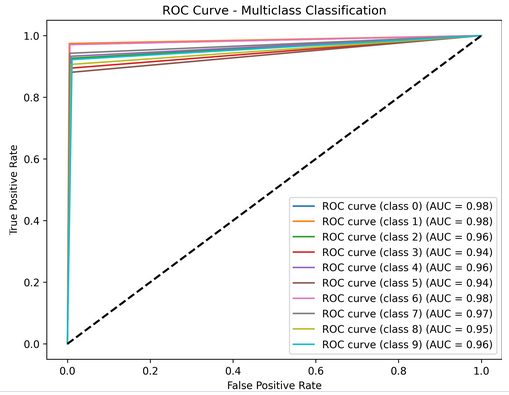
\includegraphics[width=0.6\textwidth]{rocc_component.png}
        \caption{Previsualización del componente show\_roc\_curve}
        \label{fig:roc_curve}
    \end{figure}
\end{itemize}

\paragraph{Componentes de utilidad}
\begin{itemize}
    \item \textbf{seed\_all:} Fija la semilla de todos los generadores de números aleatorios
    disponibles en la librería de Python. Se puede especificar la semilla a utilizar. También
    fija la semilla de las librerías de TensorFlow, PyTorch y Numpy si están disponibles.
    \item \textbf{get\_logger:} Devulve un objeto de tipo logger que se puede utilizar para
    imprimir mensajes en la consola en un formato específico. El formato del logger sigue la
    siguiente sintaxis \textit{\%(asctime)s - \%(levelname)s - \%(module)s - \%(message)s} 
\end{itemize} 

\paragraph{Componentes de métricas}
\begin{itemize}
    \item \textbf{mean\_absolute\_percentage\_error:} Error medio absoluto porcentual (MAPE) 
    calcula el error porcentual absoluto medio entre dos conjuntos de valores, la primera 
    entrada son los valores reales y la segunda son los valores predichos.
\end{itemize}

\subsubsection{Resultados basados en los desarrollos}
A continuación, se presenta una tabla con la recopilación de los tiempos. La tabla \ref{tabla:result-time-scores} 
muestra unicamente el tiempo de desarrollo de los proyectos, sin tener en cuenta
otros factores como el tiempo en la creación de nuevas plantillas o componentes.

\begin{table}[h!]
    \centering
    \begin{tabular}{|l|c|c|c|}
    \hline
    \textbf{Proyecto} & \textbf{Tiempo} & \textbf{Nuevos componentes} & \textbf{Utiliza plantilla} \\
    \hline
    Predicción Temperatura & 3h 30min & 5 & No \\
    \hline
    Consumo Energético & 1h 40min & 1 & Si \\
    \hline
    Clasificación Estación & 2h 00min & 2 & No \\
    \hline
    Estación SKTime & 0h 30min & 0 & Si \\
    \hline
    Anomalías Taxi & 2h 30min& 2 & No \\
    \hline
    Temperatura AutoML & 1h 20min & 1 & Si \\
    \hline
    \end{tabular}
    \caption{Comparación de tiempos de desarrollo de proyectos}
    \label{tabla:result-time-scores}
\end{table}

La utilización de plantillas y componentes reutilizables dentro del nuevo 
marco tecnológico ha demostrado reducir significativamente los tiempos de 
desarrollo de los proyectos. Los proyectos que usaron plantillas, 
presentaron tiempos de desarrollo más bajos en comparación con aquellos que no 
las usaron. Esto sugiere que las plantillas mejora eficientemente y puede ser 
recomendado para futuros desarrollos para minimizar el tiempo invertido en proyectos.\medskip

Otro de los aspectos a destacar es que ha medida que se incorporan nuevos componentes 
al sistema de conocimiento cada vez es más complicado encontrar nuevos que aporten
valor al sistema. Este fenómeno se puede deber a que las necesidades de los proyectos
son bastante similares y los componentes que se han creado hasta ahora cubren la mayoría
de los casos de uso. Por otro lado, es posible que a medida que se vayan incorporando
nuevos miembros al sistema, estos aporten nuevas ideas que permitan la creación de nuevo
conocimiento que no se había contemplado hasta ahora.\medskip

Por último, se ha observado que el uso de técnicas de AutoML ha permitido mejorar
la precisión de los modelos de \textit{forecasting}. Esto se debe a la capacidad de
probar no solo diferentes tipos de algoritmos de \textit{Machine Learning} sino también el uso
de distintas combinaciones de hiperparámetros. 